%% sample file for Modelica 2021 Conference paper
%% Copyright  Modelica Association
%
% This work may be distributed and/or modified under the
% conditions of the LaTeX Project Public License, either version 1.3
% of this license or (at your option) any later version.
% The latest version of this license is in
%   http://www.latex-project.org/lppl.txt
% and version 1.3 or later is part of all distributions of LaTeX
% version 2005/12/01 or later.
%
% This work is 'maintained' on GitHub:
%   https://github.com/modelica-association/conference-templates
%
% The Current Maintainers are: @akloeckner, @dietmarw, @bernhard-thiele
% With additions by @casella, @sjoelund
%
% This work consists of all files in the GitHub repository except
% a) The files indicated by .gitignore files
% b) The GitHub management files .gitignore, *.md
%
% This class is created from the template for the Modelica 2021 conference

%%% Use the more modern biber and biblatex for Unicode and @online support
\documentclass{modelica}
\addbibresource{example-paper.bib}

\hypersetup{%
  pdftitle  = {Latex Template for the International Modelica Conference},
  pdfauthor = {Author Name1, Author Name2},
  pdfsubject = {14th International Modelica Conference 2021},
  pdfkeywords = {Modelica, confercence, LaTeX, template},
  colorlinks,
  linkcolor=black,
  urlcolor=black,
  citecolor=black,
  pdfpagelayout = SinglePage,
  pdfcreator = pdflatex,
  pdfproducer = pdflatex}

% begin the document
\begin{document}
\thispagestyle{empty}

\title{Int. Modelica Conf. 2021 Paper Title}
\author[1]{Author Name}
\author[1]{Author Name}
\author[2]{Author Name}
\affil[1]{Department, University, Country, {\small\texttt{\{name1,name2\}@university.org}}}
\affil[2]{Company, Country, {\small\texttt{name3@company}}}

% \title{\textbf{Int. Modelica Conf. 2021 Paper Title}}
% \author{{\large
% Author Name$^1$ \quad Author Name$^1$ \quad Author Name$^2$\vspace{2mm}\\
%   {}$^1$Department, University, Country, \textsf{\{name1,name2\}@university.org}\\
%   {}$^2$Company, Country, \textsf{name3@company}}

\maketitle\thispagestyle{empty} %% <-- you need this for the first page
\abstract{%
This template shows the guidelines on how to create a paper to be submitted to the International Modelica Conference.
Please visit {\small\url{https://github.com/modelica-association/conference-templates}} if there are any questions or suggestions regarding this template.
}

\noindent\emph{Keywords: keyword1, keyword2}

\section{Introduction}

In the following section, short style guidelines are given.

\subsection{Title and Authors}
Words should be capitalized in the title, e.g., ``This is an Example of
a Correct Title''.  The author information should at least include
name, affiliation (department, university, country). Addresses and
emails are optional but strongly recommended.

\subsection{Abstract and Keywords}

The abstract should be written as one paragraph. It is not recommended
to exceed 150 words.

Appropriate keywords describing the content of the paper should be
supplied as a comma separated list.

\subsection{Fonts}

For all standard body text \emph{Times New Roman} with regular font style, and font size 10.5pt should be used. To emphasize a text or a word, use \emph{italic font style}. For verbatim text embedded in running text, including code fragments, use the style {\small\texttt{texttt}} with font Courier New with size 9.5pt should be used (1pt smaller than running text)

For separate Modelica code examples, use the style font size 9~pt.
Similar for non-Modelica code examples.
For formatting Modelica code this template used the listings definitions from {\small\url{https://github.com/modelica-tools/listings-modelica}} (included in the package).
Code listings are cross-referenced as for example \autoref{lst:while-loop}.

\begin{lstlisting}[caption=A while loop,label=lst:while-loop]
while x<20 loop
  x := x+y*2;
end while;
\end{lstlisting}

\subsection{Lists}

Bullets should be created with the \texttt{itemize} environment:
\begin{itemize}
\item The first text item.
\item The second text item.
\end{itemize}
Numbered items should be created with the \texttt{enumerate} environment:
\begin{enumerate}
\item The first text item.
\item The second text item.
\end{enumerate}

\section{Figures}

Figures should be numbered and include a description text. All figures
should be referenced within the body text using the capitalized word
``Figure'' followed by the figure number. For example,
\autoref{fig:figure1} shows a figure located inside one column and
\autoref{fig:figure2} illustrates how a figure can span over two
columns.
You should use vector graphics such as (SVG, EPS, PDF, EMF) rather than raster images such as (JPG, PNG) whenever possible.
Photographs naturally should be raster images.
Rather than using print screen you can often use the "Print" option of software to produce a PDF and especially plots can often be printed or exported to tools that produce vector graphic plots.
If you need to convert vector images between different formats, \textcite{inkscape} is very handy.

\begin{figure}[b]
\centering
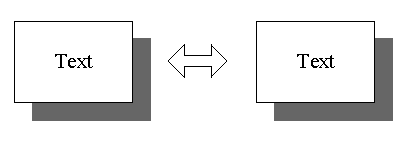
\includegraphics[width=0.4 \textwidth]{resources/figure1}
\caption{An example of a figure that fits into one column.}
\label{fig:figure1}
\end{figure}

\begin{figure*}[t]
\centering
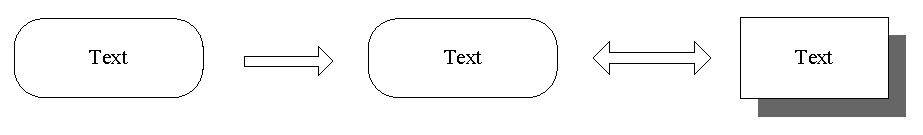
\includegraphics[width=0.9 \textwidth]{resources/figure2}
\caption{Another example of a figure that spans over two columns.}
\label{fig:figure2}
\end{figure*}

\section{Equations}
Equations should be numbered on the right side, such as:
\begin{align}
a_1& =b_1+c_1 \label{eq:a1} \\
a_2& =b_2+c_2-d_2+e_2 \label{eq:a2}
\end{align}
Equations are cross-referenced as \autoref{eq:a1} and \autoref{eq:a2}.

\section{Tables}

\autoref{tab:extab} illustrates the use of tables.
It uses the \texttt{booktabs} package which provides improved typesetting of tables and \texttt{numprint} for the thousands separator.
\begin{table}[htbp]
  \caption{Sizes of compiler phases, lines of code.}\label{tab:extab}
  \centering
  \begin{tabular}{p{6cm}r} \toprule
      \emph{Compiler Phase} & \emph{Lines} \\
      \midrule
      FrontEnd & \numprint{92192} \\
      BackEnd & \numprint{29190} \\
      Code generation & \numprint{8957} \\
      \emph{Total size} & \emph{\numprint{130339}} \\
      \bottomrule
  \end{tabular}
\end{table}

\section{Additional meaningless text}
This section contains additional text to bring the example length to three pages



Lorem ipsum dolor sit amet, consectetur adipiscing elit. Quisque faucibus, arcu non malesuada condimentum, nibh est aliquet nunc, in tempus nisi urna id dolor. Suspendisse potenti. Sed nec accumsan massa, porttitor placerat purus. Mauris nibh tellus, lobortis ac posuere non, bibendum ut mi. Etiam et quam at arcu gravida ullamcorper. Donec eget tortor eros. Pellentesque habitant morbi tristique senectus et netus et malesuada fames ac turpis egestas. Donec quis odio tellus. Integer consequat vulputate dolor, sit amet sodales nibh dapibus eu. Quisque accumsan mauris tellus, ut sollicitudin sapien finibus in. Fusce congue, mauris vestibulum vulputate commodo, quam leo faucibus purus, id luctus augue est vitae dolor. Suspendisse id ultrices diam, eget viverra diam. Donec non sem mauris. Fusce sagittis neque justo, in mollis felis luctus in. Pellentesque tincidunt mauris a feugiat accumsan. Nulla eget sem nisi.

Cras enim tortor, luctus et vulputate vitae, condimentum quis massa. Nullam fermentum, lectus a mattis laoreet, eros nunc interdum nibh, in commodo justo ipsum quis mauris. Donec imperdiet faucibus lacinia. Phasellus malesuada porta arcu, nec molestie dui posuere quis. Donec porttitor, tellus id egestas feugiat, dui quam luctus dui, vel ornare metus lorem sit amet ex. Sed bibendum convallis condimentum. Vivamus eu consectetur felis. Sed turpis nisi, malesuada id augue eu, semper pulvinar metus. Nullam id ante sed mauris bibendum iaculis. Proin rhoncus justo mauris, vel iaculis nunc rhoncus in. Aenean nec lectus non eros mollis lacinia. Fusce at massa in nunc scelerisque egestas. Nulla in turpis ante. Quisque luctus at velit vitae iaculis.

Etiam nec sapien risus. Duis lorem felis, varius et purus at, malesuada pellentesque enim. Fusce lobortis ac elit eget feugiat. Nam purus libero, aliquam eu urna quis, volutpat eleifend leo. Ut a volutpat felis. Praesent lobortis sapien nunc, vel mattis nisi laoreet et. Praesent elementum ex a fringilla pulvinar. Vestibulum condimentum elementum pharetra. Mauris condimentum tempus risus, tincidunt viverra velit. Proin dictum ligula lectus, vitae euismod ligula rutrum non. Nunc non enim ultrices, sollicitudin nibh ut, lacinia ex. Nullam ac ullamcorper ante. Nullam tristique laoreet enim, sit amet suscipit risus imperdiet non. Vivamus id turpis egestas, viverra mauris non, sagittis purus.

Phasellus eget lobortis magna. Mauris faucibus elit eget magna gravida, nec ultrices eros consectetur. Quisque porttitor tincidunt nunc vitae gravida. Vestibulum laoreet tempus feugiat. Etiam sit amet molestie urna. Praesent libero nisi, sollicitudin accumsan ullamcorper auctor, mollis sed nulla. Pellentesque consequat, nibh ac ultrices pulvinar, tortor enim aliquet augue, non facilisis lorem arcu nec justo. Vestibulum posuere a metus nec aliquam. Quisque commodo, neque rhoncus scelerisque viverra, velit sapien mollis tellus, et scelerisque est massa vitae risus. Cras sollicitudin nisl sit amet suscipit lobortis. Vivamus sit amet arcu rhoncus, varius nisi id, viverra leo. In hac habitasse platea dictumst. Pellentesque placerat sem rutrum condimentum elementum. Cras euismod augue et luctus facilisis.

Phasellus feugiat vehicula dolor, eu dapibus ex aliquam vitae. Nunc tortor magna, lacinia id consectetur et, lacinia id enim. Nunc at consectetur odio, ac blandit ex. Aliquam pharetra mi vitae mauris maximus, in sagittis orci ultrices. Curabitur sagittis tortor sem, ornare aliquet dolor congue vitae. Etiam sed nunc ut leo gravida commodo. Maecenas rhoncus odio id tortor blandit dignissim. Proin sed tincidunt metus, eget pharetra odio. Nullam et imperdiet nisl. Praesent sagittis, nunc vel laoreet tristique, quam lorem varius quam, ut varius est purus sit amet tellus. Cras ac massa neque. Aliquam pulvinar auctor elit in tincidunt.

Maecenas iaculis odio at purus porta, ac tincidunt libero interdum. Aliquam sed sapien leo. Duis malesuada pharetra ex, eu vulputate est mattis at. Cras et lacus ac quam pellentesque efficitur et ut purus. Sed sed eros non justo gravida volutpat sed non libero. Proin imperdiet pretium mattis. Quisque sapien ex, dignissim vitae eleifend id, hendrerit at neque. Sed ultrices ante purus, nec hendrerit urna congue sed. Maecenas malesuada bibendum velit, convallis varius sapien volutpat vel. Ut malesuada pretium orci, eu elementum leo malesuada id. Etiam ullamcorper lobortis imperdiet. Phasellus ornare bibendum ante vitae vestibulum. Integer eu arcu sit amet ligula elementum blandit.

Praesent suscipit, purus eget tempor placerat, lectus lorem facilisis odio, at sagittis sapien leo ac justo. Etiam suscipit quis nisl vel posuere. Suspendisse vulputate arcu eu metus maximus, vitae scelerisque elit porta. Aliquam pulvinar libero in libero interdum iaculis. In metus ligula, vestibulum et ligula eu, sagittis mattis odio. Duis in convallis lorem. Nam at pharetra est. Donec eleifend fringilla odio vitae placerat. Integer sit amet eros eget odio condimentum placerat sit amet sed purus. Nulla at ultrices velit. Etiam ornare, purus non lacinia ullamcorper, nunc augue interdum magna, quis laoreet ante risus id sapien.

Aenean id leo gravida, sodales sem ut, imperdiet mauris. Proin pellentesque libero laoreet libero volutpat, quis euismod nibh commodo. Nam et dui vel augue convallis aliquam. Mauris magna diam, ultricies eget placerat porttitor, hendrerit non mi. Quisque pulvinar varius ex, sollicitudin vestibulum est cursus eu. Sed lobortis volutpat massa sed bibendum. Cras rutrum, sem sit amet iaculis egestas, nisi turpis vehicula ipsum, eget congue risus enim vehicula turpis. Curabitur sit amet tortor vitae augue tempor consequat.

\section{Bibliographic References}
The bibliographic reference list are shown at the end of the paper;
starting with an unnumbered heading \emph{``References''}. The list of
references should be sorted in alphabetic order according to the first
author's surname.
The first author's name is printed surname first and subsequent authors are printed with the first name first.

Citations are stated within the body text using the name of the
reference enclosed within parentheses, e.g., \cite{Pantelides:1988}. If
more than one reference is cited at the same place, the list should be
sorted, separated by semicolons and within parentheses, e.g.,
\cite{DuffReid:1978,Pierce:2002,Plotkin:1981}.
It is also possible use the textcite command to include a reference more naturally in the text: \textcite{Pantelides:1988} wrote something interesting in his paper.
If there is a DOI for the reference, use it instead of URLs in the bibliography.

Citations for relevant Modelica language specifications (MLSs) are provided as
MLSv32r2 \cite{MLSv32r2}, MLSv33r1 \cite{MLSv33r1}, and MLSv34 \cite{MLSv34}.

All entries in the reference list should be cited in the manuscript.

In order to populate the bibliography with different kinds of entries to show how they should be printed, here are some additional citations:

\begin{itemize}
\item A book \cite{Kernighan:1988}.
\item A conference paper \cite{colaco:2003}.
\item A couple of fake PhD, MSc, and BSc thesis \cite{Doe:PhD,Doe:MSc,Doe:BSc}.
\end{itemize}

\section*{Acknowledgements}

This work has been supported by X (grant numbers aaaa, bbbb); Y (grant number cccc) and Z (grant number dddd).
The authors would also like to thank A and B for their support with implementation of the software.

\printbibliography

\end{document}
